\documentclass{article}[12pt]

\usepackage{graphicx}

\begin{document}
	
\section{9/20 transit}
	
\begin{table}[h]
	\begin{center}
	\begin{tabular}{|c | c | c | c | c | c|}
		\hline
		Star Name & Start & Mid & End & Duration & Magnitude Dip \\
		\hline
		\hline
		HD 189733 A & 9:25pm & 10:25pm & 11:26pm & 2.02h & 0.022 mag\\
		\hline
	\end{tabular}
	\end{center}
\end{table}

\begin{figure}[h]
	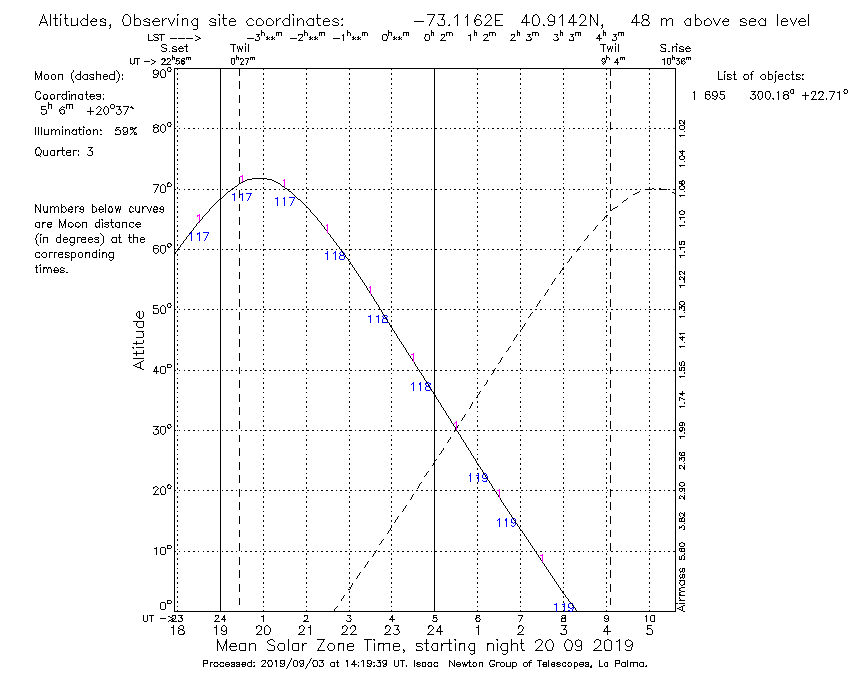
\includegraphics[width=\linewidth]{695_9_20.png}
\end{figure}

\newpage

\section{9/23 transit}

\begin{table}[h]
	\begin{center}
		\begin{tabular}{|c | c | c | c | c | c|}
			\hline
			Star Name & Start & Mid & End & Duration & Magnitude Dip \\
			\hline
			\hline
			GSC 03549-02811 & 8:46pm & 10:00pm & 11:14pm & 2.47h & 0.016 mag\\
			\hline
		\end{tabular}
	\end{center}
\end{table}

\begin{figure}[h]
	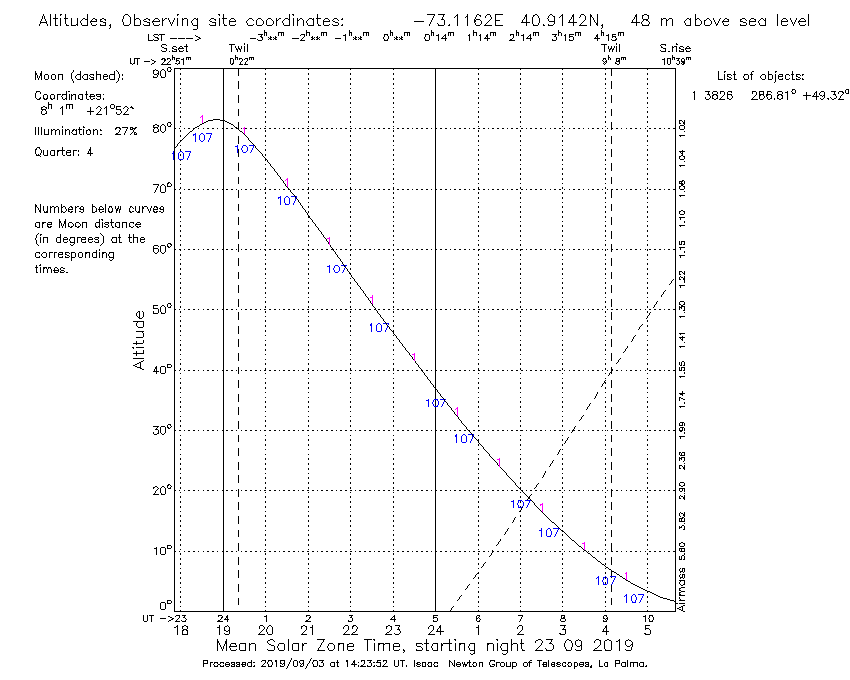
\includegraphics[width=\linewidth]{3826_9_23.png}
\end{figure}

\newpage

\section{10/01 transit}

\begin{table}[h]
	\begin{center}
		\begin{tabular}{|c | c | c | c | c | c|}
			\hline
			Star Name & Start & Mid & End & Duration & Magnitude Dip \\
			\hline
			\hline
			WASP-32 & 10:30pm & 11:51pm & 1:13am & 2.72h & 0.012 mag\\
			\hline
		\end{tabular}
	\end{center}
\end{table}

\begin{figure}[h]
	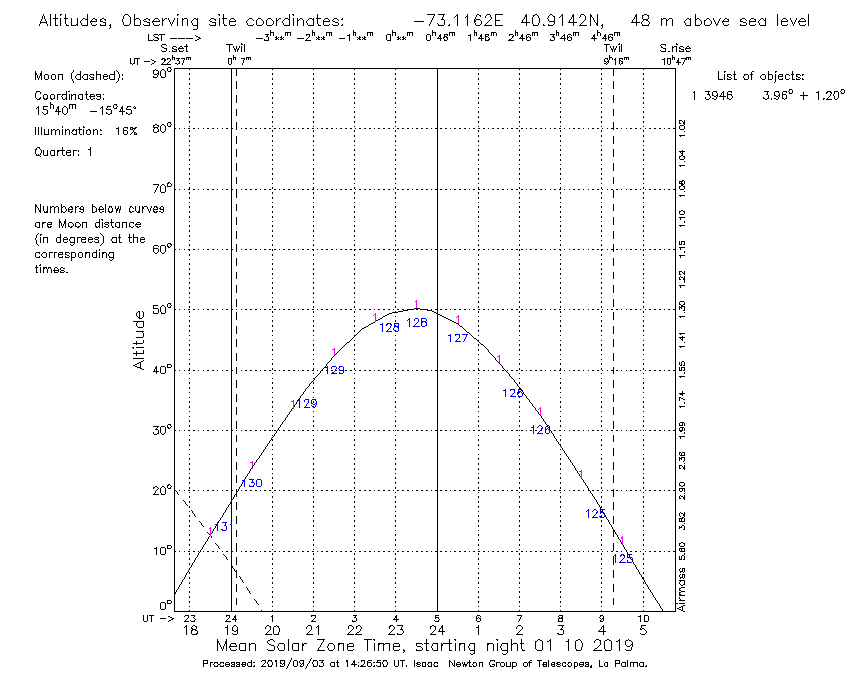
\includegraphics[width=\linewidth]{3946_10_01.png}
\end{figure}

\end{document}